% Kopfzeile beim Kapitelanfang:
\fancypagestyle{plain}{
%Kopfzeile links bzw. innen
\fancyhead[L]{\Large Vorlesung 23 (13.01.2013)}
%Kopfzeile rechts bzw. außen
\fancyhead[R]{}}
%Kopfzeile links bzw. innen
\fancyhead[L]{\Large Vorlesung 23 (13.01.2014)}
%Kopfzeile rechts bzw. außen
\fancyhead[R]{}
% **************************************************
\section{Satz}\label{12.5}
\en{
\item Für $z \in \C$ gilt: $e^z=1 \Lra z = 2k \pi i$ mit $k \in \Z$
\item $2 \pi$ ist die kleinste Periode von $\sin, \cos$
}

\subsection*{Beweis}
\en{
\item "`$\La$"' siehe oben.\\
"`$\Ra$"': Sei $e^z=1, z=x+iy$ ($x,y \in \R$).\\
$\Ra 1=|e^z|=|e^x \cdot e^{iy}| = e^x \cdot \underbrace{|e^{iy}|}_{=1} = e^x \Ra x=0$\\
$\Ra 1=e^z=e^{iy}=\cos y + i \cdot \sin y \Ra \cos y=1, \sin y = 0$\\
$\Ra y=k \pi, k \in \Z$ gerade
$\Ra z=2l \pi i, l \in \Z$
\item Angenommen, $\cos$ (und damit auch $\sin$) hat eine Periode $p$ mit $0 < p < 2 \pi$.\\
$\Ra e^{ip} = \cos p + i \cdot \sin p = \underbrace{\cos 0}_{=1} + i \cdot \sin 0 = 1$ \wspruch zu (1)
} \qed

\section{Definition: Tangens, Cotangens}\label{12.6}
$\tan x := \frac{\sin x}{\cos x}, x \in \R \setminus \{\frac{\pi}{2} + k \pi, k \in \Z\}$\nl
$\cot x := \frac{\cos x}{\sin x}, x \in \R \setminus \{k \pi, k \in \Z\}$\nl
$\tan x, \cot x$ sind ungerade Funktionen und $\pi$-periodisch.\\
$\tan: \left(-\frac{\pi}{2},\frac{\pi}{2}\right) \to \R$ ist differenzierbar, s.m.w. und bijektiv (Übung).

\subsection*{Graph von Tangens}
\begin{tikzpicture}
\draw[->] (-4,0)--(4,0);
\draw[->] (0,-4)--(0,4);
\draw[color=blue,domain=-4:-1.81577] plot (\x, {tan(deg(\x))});
\draw[color=blue,domain=-1.32582:1.32582] plot (\x, {tan(deg(\x))});
\draw[color=blue,domain=1.81577:4] plot (\x, {tan(deg(\x))});
\draw[color=blue,dashed] (1.57079,-4)--(1.57079632679,4);
\draw[color=blue,dashed] (-1.57079,-4)--(-1.57079632679,4);
\draw (-1.57079,-0.5) node[right] {$-\frac{\pi}{2}$};
\draw (1.57079,-0.5) node[left] {$\frac{\pi}{2}$};
\draw (-3.14159,0) node[below] {$-\pi$};
\draw (3.14159,0) node[below] {$\pi$};
\end{tikzpicture}

\newpage

\section{Definition: Arcus-Funktionen}\label{12.7}
\en{
\item $\sin: \left[-\frac{\pi}{2},\frac{\pi}{2}\right] \to [-1,1]$ ist stetig (sogar differenzierbar), s.m.w. und bijektiv.\nl
\begin{tikzpicture}
\draw[->] (-2,0)--(2,0);
\draw[->] (0,-1.5)--(0,1.5);
\draw[color=blue,domain=-1.57079:1.57079] plot (\x, {sin(deg(\x))});
\draw[dashed,domain=-2:-1.57079] plot (\x, {sin(deg(\x))});
\draw[dashed,domain=1.57079:2] plot (\x, {sin(deg(\x))});
\draw[dashed] (-1.57079,-1)--(-1.57079,0) node[above] {$-\frac{\pi}{2}$};
\draw[dashed] (1.57079,1)--(1.57079,0) node[below] {$\frac{\pi}{2}$};
\draw (0,1) node {$-$};
\draw (0,-1) node {$-$};
\end{tikzpicture}\nl
Denn: $\sin' x = \cos x > 0 \forall x \in \left(-\frac{\pi}{2},\frac{\pi}{2}\right)$\\
$\underset{\text{\ref{11.13}}}{\Ra} \sin$ s.m.w. auf $\left[-\frac{\pi}{2},\frac{\pi}{2}\right]$.\\
$\sin \left(\pm \frac{\pi}{2}\right) = \pm 1$\\
ZWS $\Ra$ Bijektivitätsaussage\nl
Umkehrfunktion: $\arcsin: [-1,1] \to \left[-\frac{\pi}{2},\frac{\pi}{2}\right]$, der \underline{Arcus-Sinus}\nl
\begin{tikzpicture}
\draw[->] (-2,0)--(2,0);
\draw[->] (0,-2)--(0,2);
\draw[color=red,domain=-1:1] plot (\x, {asin(\x)/360*2*pi});
\draw (-1,0) node {$|$} node[below] {$-1$};
\draw (1,0) node {$|$} node[below] {$1$};
\draw (0,-1.57079) node {$-$} node[left] {$-\frac{\pi}{2}$};
\draw (0,1.57079) node {$-$} node[left] {$\frac{\pi}{2}$};
\end{tikzpicture}\nl
Ableitung: Satz \ref{11.8} $\Ra \arcsin'(y) = \frac{1}{\sin'(x)} = \frac{1}{\cos x}$ mit $y = \sin x$, sofern $\sin' x = \cos x \neq 0$\\
$\cos x > 0 \forall x \in \left(-\frac{\pi}{2},\frac{\pi}{2}\right), \cos \left(\pm \frac{\pi}{2}\right) = 0$\\
$\cos x = + \sqrt{1 - \sin^2 x} = \sqrt{1-y^2} \forall x \in \left(-\frac{\pi}{2},\frac{\pi}{2}\right)$\\
$\Ra$ \fbox{$\arcsin'(y) = \frac{1}{\sqrt{1-y^2}}$} $\forall y \in (-1,1)$\\
(nicht differenzierbar in $y = \pm 1$, Graph hat dort vertikale Tangente)
\newpage
\item $\cos: [0,\pi] \to [-1,1]$ ist stetig, s.m.f. und bijektiv (analog)\nl
\begin{tikzpicture}
\draw[->] (-2,0)--(4,0);
\draw[->] (0,-1.5)--(0,1.5);
\draw[color=blue,domain=-2:3.14159] plot (\x, {cos(deg(\x))});
\draw[dashed,domain=3.14159:4] plot (\x, {cos(deg(\x))});
\draw (1.57079,0) node[below] {$\frac{\pi}{2}$};
\draw[dashed] (3.14159,-1)--(3.14159,0) node[above] {$\pi$};
\draw (0,1) node {$-$};
\draw (0,-1) node {$-$};
\end{tikzpicture}\nl
Umkehrfunktion: $\arccos: [-1,1] \to [0, \pi]$, der \underline{Arcus-Cosinus}\nl
\begin{tikzpicture}
\draw[->] (-2,0)--(2,0);
\draw[->] (0,-0.5)--(0,3.5);
\draw[color=red,domain=-1:1] plot (\x, {acos(\x)/360*2*pi});
\draw (-1,0) node {$|$} node[below] {$-1$};
\draw (1,0) node {$|$} node[below] {$1$};
\draw (0,3.14159) node {$-$} node[left] {$\pi$};
\draw (0,1.57079) node {$-$} node[left] {$\frac{\pi}{2}$};
\end{tikzpicture}\nl
\item Umkehrfunktion von $\tan: \left(-\frac{\pi}{2},\frac{\pi}{2}\right) \to \R$:\\
$\arctan: \R \to \left(-\frac{\pi}{2},\frac{\pi}{2}\right)$, ebenfalls differenzierbar und s.m.w., der \underline{Arcus-Tangens}\nl
\begin{tikzpicture}
\draw[->] (-3.5,0)--(3.5,0);
\draw[->] (0,-1.5)--(0,1.5);
\draw[color=red,domain=-3.14159:3.14159] plot (\x, {atan(\x)/360*2*pi});
\draw (-3.14159,0) node {$|$} node[below] {$-\pi$};
\draw (3.14159,0) node {$|$} node[below] {$\pi$};
\draw (0,-1) node {$-$} node[left] {$-1$};
\draw (0,1) node {$-$} node[left] {$1$};
\end{tikzpicture}\nl
$\tan \frac{\pi}{4} = 1$\\
$\arctan 1 = \frac{\pi}{4}$\\
\fbox{$\arctan' y = \frac{1}{1+y^2}$} (Übung)
}

\newpage

\phantomsection
\addcontentsline{toc}{section}{Polarkoordinaten}
\section*{Polarkoordinaten}
Erinnerung: $\varphi \in \R \Ra \left|e^{i \varphi}\right| = 1$

\section{Satz}\label{12.8}
Jedes $z \in \C$ ist darstellbar als $z = re^{i \varphi}$ mit $r = |z| \ge 0, \varphi \in \R$\nl
Für $z \neq 0$ ist $\varphi$ eindeutig bis auf Addition von $2 k \pi, k \in \Z$\\
$(r,\varphi)$: \underline{Polarkoordinaten} von $z$\\
$\varphi$: \underline{Argument} von $z$. Übliche Wahl: $\varphi \in (-\pi, \pi]$, oder $\varphi \in [0, 2 \pi)$\nl
\begin{tikzpicture}
\draw[->] (-0.5,0)--(3,0);
\draw[->] (0,-0.5)--(0,3);
\draw[color=blue] (0,0)--(2.5,2.5) node {$\bullet$} node[right] {$z$};
\draw (1.25,1.25) node[right] {$r=|z|$};
\draw[color=red,->](0.5,0) arc (0:45:0.5);
\draw[color=red] (0.8,0.3) node {$\varphi$};
\end{tikzpicture}

\subsection*{Beweis}
$z = 0 \Ra r = 0, \varphi$ beliebig\\
Sei $z \neq 0 \Ra r := |z| \neq 0, w := \frac{z}{r} \Ra |w| = 1$\\
$w = x + iy$, $x,y \in \R$, $x^2+y^2=1$, insbes. $x \in [-1,1]$\nl
Setze $\varphi := \arccos x \in [0,\pi]$.\\
$\Ra x = \cos \varphi$\\
$y = \pm \sqrt{1-x^2} = \pm \sqrt{1-\cos^2 \varphi} = \pm \underbrace{\sin \varphi}_{\ge 0}$\nl
\begin{tikzpicture}
\draw[->] (-0.5,0)--(3,0);
\draw[->] (0,-3)--(0,3);
\draw[color=blue] (0,0)--(2.5,2.5) node {$\bullet$} node[right] {$w=e^{i \varphi}$};
\draw[color=blue] (0,0)--(2.5,-2.5) node {$\bullet$};
\draw[color=red,->](0.5,0) arc (0:45:0.5);
\draw[color=red] (0.8,0.3) node {$\varphi$};
\draw[color=orange,->](0.5,0) arc (0:-45:0.5);
\draw[color=orange] (0.8,-0.3) node {$-\varphi$};
\draw (2.5,0)--(2.5,2.5);
\draw (2.5,1.25) node[right] {$y$};
\draw (2.5,-2.5) node[right] {$y < 0$};
\end{tikzpicture}
\newpage
\items{
\item[1. Fall:] $y \ge 0 \Ra y = \sin \varphi \Ra w = \cos \varphi + i \cdot \sin \varphi = e^{i \varphi}$
\item[2. Fall:] $y < 0 \Ra y = -\sin \varphi = \sin(-\varphi) \Ra w = e^{-i \varphi}$
}
Zur Eindeutigkeitsaussage: Sei $z = r \cdot e^{i \varphi} = e \cdot e^{i \psi}, z \neq 0$\\
$\underset{r \neq 0}{\Ra} e^{i(\varphi-\psi)} = 1 \underset{\text{Satz \ref{12.5}}}{\Ra} \varphi - \psi = 2k \pi, k \in \Z$\nl
% TODO: Graph 12.8 (3)
$e^{i \varphi} = e^{i (\varphi+2 \pi)}$\nl
Polarkoordinaten sind praktisch für Multiplikation in $\C$:\\
$z = r \cdot e^{i \varphi}, w = s \cdot e^{i \psi} \Ra zw = r \cdot s \cdot e^{i(\varphi+\psi)}$\\
Multipliziere die Beträge, addiere die Argumente!

\section{Satz}\label{12.9}
Die Gleichung $z^n = 1$ ($n \in \N$) hat in $\C$ genau die $n$ Lösungen\\
$z_k = e^{2 \pi i \frac{k}{n}}, k = 0,1,\ldots,n-1$ (\underline{$n$-te Einheitswurzeln})\nl
Die $z_k$ bilden die Ecken eines regelmäßigen $n$-Ecks.\nl
Für $n=6$:\nl
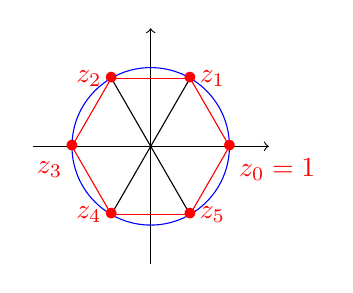
\begin{tikzpicture}
\draw[->] (-1.5,0)--(1.5,0);
\draw[->] (0,-1.5)--(0,1.5);
\draw[color=blue] (0,0) circle (1);
\draw[color=red] (1,0)--(0.5,0.8660254);
\draw[color=red] (0.5,0.8660254)--(-0.5,0.8660254);
\draw[color=red] (-0.5,0.8660254)--(-1,0);
\draw[color=red] (-1,0)--(-0.5,-0.8660254);
\draw[color=red] (-0.5,-0.8660254)--(0.5,-0.866025);
\draw[color=red] (0.5,-0.866025)--(1,0);
\draw (-0.5,0.8660254)--(0.5,-0.8660254);
\draw (0.5,0.8660254)--(-0.5,-0.8660254);
\draw[color=red] (1,0) node {$\bullet$} (1,-0.3) node[right] {$z_0=1$};
\draw[color=red] (0.5,0.8660254) node {$\bullet$} node[right] {$z_1$};
\draw[color=red] (-0.5,0.8660254) node {$\bullet$} node[left] {$z_2$};
\draw[color=red] (-1,0) node {$\bullet$} (-1,-0.3) node[left] {$z_3$};
\draw[color=red] (-0.5,-0.8660254) node {$\bullet$} node[left] {$z_4$};
\draw[color=red] (0.5,-0.8660254) node {$\bullet$} node[right] {$z_5$};
\end{tikzpicture}

\subsection*{Beweis}
Nach Fundamentalsatz der Algebra (\ref{6.8}) hat das Polynom $p(z)=z^n-1$ genau $n$ Nullstellen in $\C$.\\
Und: $z_n^k = (e^{2 \pi i \frac{k}{n}})^n = e^{2 \pi i k} = 1$ \qed

\subsection*{Bemerkung}
$z \in \C, |z| = 1 \Ra z = e^{i \varphi}, \varphi \in [0, 2 \pi)$\\
$\varphi$: Länge des Kreisbogens von $1$ bis $z$\\
$2 \pi$: Umfang des Einheitskreises\nl
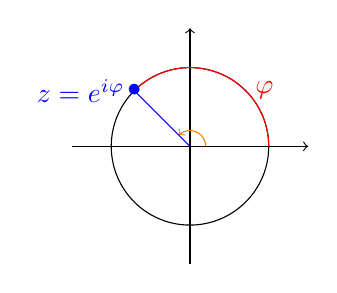
\begin{tikzpicture}
\draw[->] (-1.5,0)--(1.5,0);
\draw[->] (0,-1.5)--(0,1.5);
\draw (0,0) circle (1);
\draw[color=red](1,0) arc (0:135:1) (0.70710678,0.70710678) node[right] {$\varphi$};
\draw[color=orange,->](0.2,0) arc (0:135:0.2);
\draw[color=blue] (0,0)--(-0.70710678,0.70710678) node {$\bullet$} node[left] {$z=e^{i \varphi}$};
\end{tikzpicture}

\chapter{Gleichmäßige Konvergenz, Potenzreihen}\label{P13}
Sei $D \subseteq \R$ und $f_n: D \to \R$ ($n \in \N$) eine Folge von Funktionen mit gemeinamen Definitionsbereich $D$.

\section{Definition: Punktweise Konvergenz}\label{13.1}
$(f_n)_{n \in \N}$ konvergiert \underline{punktweise} gegen eine Funktion $f: D \to \R :\Lra \forall x \in D: f_n(x) \to f(x)$ ($n \to \infty$)\\
d.h. $\forall x \in D \forall \eps > 0 \exists N(x) \in \N: |f_n(x)-f(x)| < \eps \forall n \ge N(x)$

\subsection*{Beispiel}
$f_n(x) = x^n$ auf $D = [0,1]$ ($n \in \N$)\nl
$f(x) := \left\{\begin{array}{l l} 0 & x \in [0,1) \\ 1 & x=1 \end{array} \right.$\nl
% TODO: (vielleicht) Graph 13.1
Dann: $f_n \to f$ punktweise\\
Beachte: alle $f_n$ sind stetig, aber $f$ ist unstetig in $x = 1$!

\subsubsection*{Anschaulich}
Siehe Skript.

\section{Definition: Gleichmäßige Konvergenz (Stärkerer Konvergenzbegriff)}\label{13.2}
$(f_n)_{n \in \N}$ konvergiert \underline{gleichmäßig} auf $D$ gegen $f: D \to \R$\\
$:\Lra \forall \eps > 0 \exists N \in \N: |f_n(x)-f(x)| < \eps \forall n \ge N$ \underline{und} $\forall x \in D$

\subsection*{Beachte}
$N=N(\eps)$ unabhängig von $x \in D$ wählbar, die $f_n$ mit $n \ge N$ bleiben im Streifen der Breite $2 \eps$ um $f$.\\
Klar: $f_n \to f$ gleichmäßig $\Ra f_n \to f$ punktweise

\subsection*{Anschaulich}
Siehe Skript.
%\begin{tikzpicture}
%\draw[->] (1.5,0)--(3.5,0);
%\draw (2.5,0) node[below] {$D$};
%\draw[color=blue,domain=2:3] plot (\x, {0.5*(\x-3)^3+1});
%\draw[dashed,color=red,domain=2:3] plot (\x, {0.5*(\x-3)^3+1.3});
%\draw[dashed,color=red,domain=2:3] plot (\x, {0.5*(\x-3)^3+0.7});
%\end{tikzpicture}